%%%% NeurReps Extended Abstract track — OFFICIAL template (jmlr.cls from
%%%% the NeurReps style zip; see venue-requirements.md). This build is the
%%%% ANONYMIZED review version: per the template instructions no author
%%%% block appears at all during review; camera-ready uncomments it.
%%%%
%%%% TITLE: default per PAPER_SPRINT_PLAN.md §4 Decision 2 (PI-backed).
%%%% AUTHOR BLOCK: PENDING-USER — commented camera-ready placeholder below.
%%%%
%%%% The CFP asks for a single .tex file at submission: `make bundle`
%%%% writes the flattened bundle/rank-recruitment-ws-submission.tex from
%%%% this modular source.
\documentclass[mlabstract,onecolumn]{jmlr}

%%%%%%%%%%%%%%%%%%%%%%%%
% Watermark (review builds only; remove for camera-ready)
% (the sample zip writes hpos=300px,vpos=70px; px is a pdfTeX-only unit and
% this build engine runs XeTeX, so the equivalent bp values are used --
% 1px = 1bp at pdfTeX's default \pdfpxdimen)
\usepackage[hpos=300bp,vpos=70bp]{draftwatermark}
\SetWatermarkText{\test}
\SetWatermarkScale{1}
\SetWatermarkAngle{0}
%%%%%%%%%%%%%%%%%%%%%%%%

% The class auto-loads: amsmath, amssymb, natbib, graphicx, url, algorithm2e.
\usepackage{booktabs}

\graphicspath{{figures/}}

\newcommand{\R}{\mathbb{R}}
\newcommand{\rank}{\operatorname{rank}}
\newcommand{\recninety}{\mathrm{rec}@0.9}
\newcommand{\Kmat}{K_{\mathrm{mat}}}
\newcommand{\Vmat}{V_{\mathrm{mat}}}

%%%% DON'T CHANGE %%%%%%%%%
\jmlrvolume{}
\firstpageno{1}
\editors{Under Review for the NeurReps Workshop}
\jmlryear{2026}
\jmlrworkshop{Symmetry and Geometry in Neural Representations}
%%%%%%%%%%%%%%%%%%%%%%%%%%%

\title[When the Gradient Sees Rank]{When the Gradient Sees Rank: Provable
Necessity, Causal Recruitment, and Exact Composition in Trained Matrix
Memories}

% CAMERA-READY ONLY (PENDING-USER): uncomment and fill after acceptance.
% \author{\Name{Author Name(s) TBD} \Email{email@TBD}\\
% \addr Affiliation TBD}

\begin{document}

\maketitle

\begin{abstract}
Matrix-valued fast-weight memories make rank a structural budget: the
directions a state spans bound what it can bind and compose. A recent
negative result reported that a matrix latent bolted onto a
vector-pretrained reasoner never uses its rank, but the probed task admits
a rank-1 solution, leaving the general question open. We answer it on
testbeds where the exact solution provably requires
$\rank(Z) \geq K$ and where every rank-evading shortcut is closed by
construction: the readout is pinned to exact continuous recovery, since
argmax decoding lets a rank-$m$ memory store roughly $md$ associations; a
single-matrix-state bottleneck forecloses position decomposition; and no
cell is called dead without re-testing at 2--2.5$\times$ budget. Under
these conditions gradient descent recruits the rank the task demands in
this architecture family:
learned effective rank tracks $K$ across the tested grid (Spearman
$\rho = 1.0$ at $d = 16$),
% <!-- evidence: R1 -->
train-time rank caps show a causal step at $k \approx K$ (at $d = 8$,
$K = 4$: rank 3 gives at most 0.0004 recovery, rank 4 gives 0.97),
% <!-- evidence: R2 -->
and the trained operator composes exactly through 21-fold self-application
in four of five seeds.
% <!-- evidence: R3 -->
An entity-subspace decomposition supplies the mechanism, restricted rank
exactly $K$ on the key subspace,
% <!-- evidence: R5 -->
and in the single converged rank-starved seed, the depth-decay curve is
predicted from its eigenspectrum alone.
% <!-- evidence: R4 -->
\end{abstract}

\begin{keywords}
effective rank, fast weights, associative memory, composition
\end{keywords}

\section{Introduction}
\label{sec:intro}

Matrix-valued latents, in continuous chain-of-thought models
\citep{hao2024coconut} and fast-weight architectures broadly
\citep{schlag2021linear}, carry a structural observable a vector does
not have: the \emph{rank} of the state, which should track how many
items the state holds and, when constrained below what the task needs,
destroy performance.
A recent negative result tested this on a matrix-CODI model (a
$d \times d$ latent bolted onto a vector-pretrained GPT-2) and found
rank-$k$ truncation curves flat across four training regimes and four
readouts \citep{larson2026gradient}; its own stated confound is that
ProsQA admits a rank-1 solution, so flatness says nothing about tasks
that provably require rank. We close the confound: matrix-native
models trained from scratch on tasks whose exact solutions carry a
provable $\rank(Z) \geq K$ lower bound, under a readout and
architecture built so nothing short of genuine rank recruitment can
pass. The contributions: the \emph{teeth} that keep the
bound a necessity result (\S\ref{sec:setup}); recruitment of rank
tracking $K$ and its causal necessity under train-time caps
(\S\ref{sec:recruit}); exact composition to depth 21, its
invariant-subspace mechanism, and the depth-amplification signature
(\S\ref{sec:compose}); and an exactness
frontier in $d$ with a budget-extension rule (\S\ref{sec:frontier}).

\section{The Bound and the Teeth That Keep It a Bound}
\label{sec:setup}

\textbf{Task and bound.} Each episode presents $K$ key$\to$value
bindings, then queries one; keys and values are fresh per episode
(Gaussian, normalized, or exactly orthonormal following
\citealp{mezzadri2007random}), so evaluation uses never-seen bindings. Exact recovery $Z k_j = v_j$
for $K$ bindings with linearly independent keys and values forces
$Z \Kmat = \Vmat$, hence the classical bound
$K = \rank(\Vmat) = \rank(Z \Kmat) \leq \rank(Z)$
\citep{kohonen1972correlation,anderson1972simple}. We measure whether a
trained, bottlenecked model \emph{discovers} this rank under plain SGD,
and whether it is causally load-bearing.

\textbf{Tooth 1: exact continuous recovery, never argmax.}
\citet{nichani2025factual} construct a rank-$m$ linear memory storing
approximately $md$ associations under interference-tolerant argmax
decoding; under that rule a rank-1 state passes at every $K$ we test
and the bound collapses. We therefore pin the decoder to the linear
unbind itself, $\mathrm{pred} = Z \cdot k_j$, scored by an absolute bar
($\recninety$: the fraction of queries with $\cos > 0.9$), never an
argmax and never a learned readout that could launder rank.

\textbf{Tooth 2: a single-state bottleneck, verified behaviorally.}
``Hold $K$ items'' is satisfiable in full attention by attending to
$K$ raw-input positions at rank~1 each, so all information
funnels through one $d \times d$ state and the decoder is a pure
function of $(Z, \mathrm{query})$: after the encoder writes $Z$, the
raw-input cache is corrupted and the decode is confirmed bit-for-bit
unchanged (a gradient blank-out test, not a mask-shape check).
% <!-- evidence: R10 -->

\textbf{Model and controls.} A Transformer encoder over the binding
tokens, with $d$ learned row-reader latents producing the rows of
$Z \in \R^{d \times d}$: permutation-invariant, able to express any
rank up to $d$, and not hard-coding $\sum_j v_j k_j^\top$. Every model
is under 1M parameters (the $d = 16$ composition model: 170{,}896).
% <!-- evidence: R9 -->
Effective rank (entropy of the normalized singular-value spectrum) is
the pre-registered primary metric; the primary causal control
constrains $Z$ to rank $k$ at \emph{every training step} (spectral
projection), not post hoc.

\section{Rank Tracks $K$ and Is Causally Necessary}
\label{sec:recruit}

\textbf{Recruitment.} Without any rank term in the loss, the trained
$d{=}16$ state's effective rank rises one-for-one
with binding count across a ten-point grid from $K{=}1$ to $K{=}16$
(Spearman $\rho = 1.0$; 2.42 at $K{=}1$, 8.20 at $K{=}8$, 15.09 at
$K{=}16$), leaving the pre-registered $[0.7K, 1.3K]$ band only at
$K \leq 3$, by overshoot; beyond $K = d$ rank saturates and declines.
% <!-- evidence: R1 -->
A subsequent, larger replication sweep is directionally identical.
% <!-- evidence: R1b -->

\begin{figure}[t]
\centering
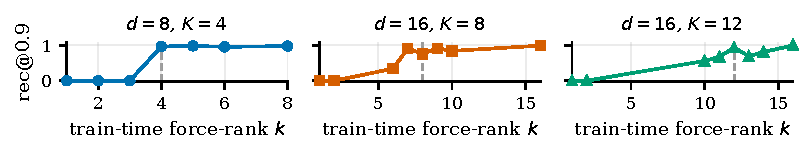
\includegraphics[width=0.92\textwidth]{fig_forcerank.pdf}
\caption{The primary, pre-registered causal test: $\recninety$ under
train-time force-rank $k$, regenerated from the archived sweep (dashed
line at $k = K$). The step lands at $k \approx K$ in every cell whose
unconstrained model reaches exact recovery.}
% <!-- evidence: R2 -->
\label{fig:forcerank}
\end{figure}

\textbf{Causal necessity.} Training with $Z$ constrained to rank $k$
throughout (Figure~\ref{fig:forcerank}): at $d{=}8, K{=}4$
the step is exact, $k \leq 3$ yields $\recninety \leq 0.0004$ and
$k = 4$ yields 0.97, a discontinuity at the provable bound.
% <!-- evidence: R2 -->
The $d{=}16$ cells show the same knee near $k \approx K$ with mild
post-knee non-monotonicity from seed noise; the replication resolves
the $K{=}12$ transition into a ragged ramp, not a clean step.
% <!-- evidence: R2b -->
The two halves answer \citet{larson2026gradient}: the earlier
rank-blindness was a property of a rank-1-solvable task, not of the
gradient.

\section{Exact Composition and the Invariant-Subspace Mechanism}
\label{sec:compose}

Binding is a single lookup; the composition variant relates the $K$
entities by one Hamiltonian $K$-cycle $\pi$, so a hop-depth-$h$ query
means recovering $v_{\pi^h(i)}$ by $h$-fold self-application of the
same trained operator, $Z^h k_i$, with no learned per-hop parameters.
Training sees hops $\{1, 2, 3\}$; evaluation adds held-out
$\{4, 5, 6\}$ and probes $\{7, 21\}$ ($d = 16$, $K = 8$, orthonormal
keys). A single full cycle is load-bearing: under a general random
permutation, nominally held-out depths collapse into trivial or
in-distribution queries modulo its short cycle lengths
(Appendix~\ref{app:period}).

\textbf{Exact composition.} 4/5 unconstrained seeds reach
$\recninety \geq 0.9996$ at every tested hop (3/5 at 1.000 throughout);
the fifth is still transitioning at budget, decaying from 0.93
($h{=}1$) to 0.16 ($h{=}7$) and 0.0001 ($h{=}21$).
% <!-- evidence: R3 -->

\begin{figure}[t]
\centering
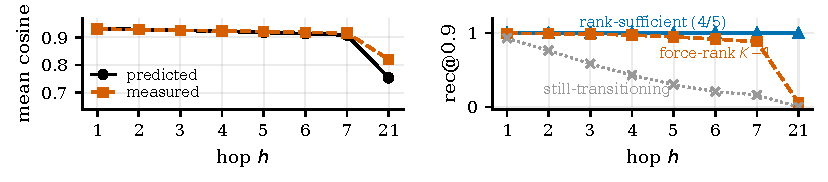
\includegraphics[width=0.92\textwidth]{fig_depth.pdf}
\caption{Depth as a spectral-exactness amplifier ($d{=}16$, $K{=}8$).
\emph{Left:} mean cosine for the converged force-rank $k{=}7{=}K{-}1$
seed against the eigenspectrum-only prediction (no raw keys).
\emph{Right:} $\recninety$ by hop for the four converged
rank-sufficient seeds (flat at 1.0), the rank-starved operator, and the
still-transitioning seed.}
% <!-- evidence: R4 -->
% <!-- evidence: R3 -->
\label{fig:depth}
\end{figure}

\textbf{Depth amplification.} At force-rank $k = K - 1$ (provably
insufficient), the one converged seed passes shallow hops at mean
cosine 0.92--0.93 ($h \leq 5$), above the 0.9 bar, and collapses only
under depth (Figure~\ref{fig:depth}): $\recninety$ falls 0.996 $\to$
0.881 $\to$ 0.060 at $h = 1/7/21$.
% <!-- evidence: R4 -->
The mechanism is spectral and predictable: from the operator's
eigenspectrum alone, predicted cosine matches the measured curve within
0.008 through $h = 7$ (Table~\ref{tab:depthcurve}).
% <!-- evidence: R4 -->


\textbf{The invariant-subspace mechanism.} Whole-matrix effective rank
of the converged solutions reads the full ambient dimension (16.0 of
$d{=}16$; stable rank 14.6--15.6); the whole-matrix number is the wrong
instrument.
% <!-- evidence: R5 -->
Block-decomposing the trained $Z$ against the ideal cycle's
$K$-dimensional entity subspace $\mathcal{E}$: the restricted operator
has effective rank 7.999--8.000 (maximum 8), matching the ideal scaled
cycle to a scale-corrected residual of 0.7--2.4\%; leakage out of
$\mathcal{E}$ is below 1.5\% of the state norm; the complement block is
full-rank and non-contractive yet dynamically invisible: a query
starting in $\mathcal{E}$ never leaves it (Table~\ref{tab:subspace},
Appendix~\ref{app:subspace}).
% <!-- evidence: R5 -->
Restricted to the subspace the task uses, ``rank tracks $K$'' holds
exactly; dead force-rank seeds fail the same restricted test, so their
collapse is real.

\section{The Exactness Frontier, and When to Trust a Dead Cell}
\label{sec:frontier}

\textbf{Budget reversals.} Three independent axes each declared a cell
dead at its first step budget before an extension reversed the verdict:
composition at $K{=}8$ (1/5 seeds converged at 20K steps; 4/5 at 40K),
% <!-- evidence: R8 -->
composition at $K \in \{12, 16\}$ (0/5 at 40K; 3/3 and 2/3 fresh seeds
at 80K),
% <!-- evidence: R6 -->
and $d$-scaling (an 8K-budget wall at $d \geq 32$ dissolving at 20K,
onset 6--16K).
% <!-- evidence: R8 -->
The rule, \emph{a cell is not dead until re-tested at 2--2.5$\times$
budget},
% <!-- evidence: R8 -->
is necessary but not sufficient: $K{=}16$'s remaining stuck
seed stayed dead through 120K steps,
% <!-- evidence: R6 -->
and the $d{=}32$ cells below plateau flat yet still fail the
pre-registered bar.
% <!-- evidence: R8 -->

\textbf{The frontier that survives} is not a trainability wall but an
\emph{exactness} frontier. Fixing $K = d/4$ at encoder width $h = 64$
(every cell confirmed flat before being read as converged), mean
recovery cosine falls monotonically across $d$:
0.877/0.909/0.915 at $d{=}32$ (three
seeds, 100K steps), 0.7196 at $d{=}48$ (100K), and 0.3882 at $d{=}64$
(150K); the exact-match metric is harsher, with $\recninety$
0.413/0.632/0.653 at $d{=}32$ (all below the pre-registered 0.7 pass
bar), 0.002 at $d{=}48$, and 0.0 at $d{=}64$.
% <!-- evidence: R7 -->
Rank recruitment and exactness separate: at $d{=}32$ recruited rank
reaches 91--97\% of target while exact recovery stalls below the bar.
% <!-- evidence: R7 -->

\section{Related Work, Limitations, and Outlook}
\label{sec:related}

\citet{nichani2025factual} is the nearest neighbor: a hand-built
existence construction under interference-tolerant argmax decoding;
this work pins the readout so that construction cannot pass, then
measures and intervenes on the rank SGD recruits
(\citealp{barnfield2026sharp} give static-memory thresholds).
\citet{nazari2026rank} and \citet{sun2026staterank} measure
effective-rank dynamics in pretrained linear-attention models
observationally (an \emph{upper} bound $\rank(S_t) \leq t$); here the
write count is controlled and necessity is causal. \citet{mishra2026m2rnn} train matrix-state RNNs on $S_3$ with no rank
measurement or intervention (their own vector-state control matches);
\citet{grazzi2025negative} and \citet{siems2025deltaproduct} (the
Householder extension of \citealp{yang2024deltanet}) characterize the
per-token \emph{transition} operator, not the trained \emph{state's}
own rank, the quantity here. Continuous-CoT capacity
results are existence constructions, not measurements
\citep{zhu2025superposition,gozeten2025cot2}; the
compositional-generalization caution
\citep{dziri2023faithfate,wang2024grokked} is met with an exact
eigenstructure match.

\textbf{Limitations.} Every experiment is synthetic and under 1M
parameters; generality at scale, and across state-writing architectures
(recurrent fast-weight, attention-readout, associative-memory), is
untested.
% <!-- evidence: R9 -->
The depth-amplification contrast rests on the single converged
force-rank-$(K{-}1)$ seed; the other two at that cell collapsed under
a documented numerical instability in the spectral-projection backward
pass, so it is a case study consistent with the spectral prediction,
not an $n{>}1$ mechanism; the $d \geq 48$ frontier cells rest on
single seeds. The registered falsifiers stand
(Appendix~\ref{app:repro}). A concurrent companion submission
(group-composition state tracking) shares no figures or tables but
restates this paper's recruitment, causal-necessity, and composition
numbers as background for its distinct contribution, a group-dimension
rank law this paper does not make.

\appendix

\section{Depth 21 Under the Single $K$-Cycle}
\label{app:period}

Under a single 8-cycle, $\pi^{21} = \pi^{21 \bmod 8} = \pi^{5}$, so the
nominal depth-21 probe shares its \emph{target} with the already-tested
depth 5; the two are not distinct group-theoretic queries. What depth 21
measures is numerical stability under 21 sequential self-applications of
the trained operator. In the four converged seeds $\recninety$ reads
$\geq 0.9996$ at both $h{=}5$ and $h{=}21$, so repeated self-application
does not amplify their residual error;
% <!-- evidence: R3 -->
in the rank-starved operator the same 16 additional applications
compound a passing shallow-hop cosine into collapse (0.947 at $h{=}5$
to 0.060 at $h{=}21$ in recovered fraction),
% <!-- evidence: R4 -->
which is exactly the amplification claim of \S\ref{sec:compose}, not a
generalization claim to unseen permutation targets.

\begin{table}[!htb]
\centering
\small
\begin{tabular}{cccc}
\toprule
$h$ & predicted $\cos$ & measured $\overline{\cos}$ & measured $\recninety$ \\
\midrule
1  & 0.9317 & 0.9303 & 0.996 \\
3  & 0.9258 & 0.9259 & 0.986 \\
5  & 0.9181 & 0.9212 & 0.947 \\
7  & 0.9089 & 0.9163 & 0.881 \\
21 & 0.7536 & 0.8206 & 0.060 \\
\bottomrule
\end{tabular}
\caption{The rank-starved ($k = 7 = K - 1$) operator's depth-decay
curve: cosine predicted from the trained operator's own eigenspectrum
(no raw keys) against the measured values, with the recovered fraction
alongside. Every hop through $h = 7$ matches within 0.008; at $h = 21$
the per-item distribution widens and the exact-match metric collapses
while mean cosine moves little.}
% <!-- evidence: R4 -->
\label{tab:depthcurve}
\end{table}

\section{Per-Seed Subspace Decomposition}
\label{app:subspace}

\begin{table}[!htb]
\centering
\small
\begin{tabular}{lccccc}
\toprule
seed & $\mathrm{effrank}(A)$ & residual & leakage (\% of $\|Z\|$) & $\mathrm{effrank}(D)$ & $\rho(D)$ \\
\midrule
s1 & 8.000 & 0.7\% & 0.44\% & 8.000 & 1.38 \\
s2 & 7.999 & 1.9\% & 1.06\% & 8.000 & 1.27 \\
s3 & 7.999 & 1.5\% & 0.87\% & 8.000 & 2.86 \\
s4 & 7.999 & 2.4\% & 1.45\% & 7.999 & 1.02 \\
\bottomrule
\end{tabular}
\caption{Entity-subspace block decomposition of the four converged
$K{=}8$ composition seeds (means over four evaluation episodes),
recomputed from the archived $Z$-dumps. $A$ is the operator restricted
to the $K$-dimensional entity subspace; residual is the scale-corrected
Frobenius distance to the ideal cycle after fitting the single isotropic
scale that cosine scoring cannot see; leakage is the cross-block norm
$\|C\|$ as a fraction of $\|Z\|$; $D$ is the complement block, full-rank
and non-contractive ($\rho(D) \geq 1$) yet never visited by a query
trajectory that starts in the entity subspace.}
% <!-- evidence: R5 -->
\label{tab:subspace}
\end{table}

\section{Reproducibility}
\label{app:repro}

Training, evaluation, and analysis code is available at
\url{https://anonymous.4open.science/} (anonymized for review). Raw
per-run JSON archives (dense training-step checkpoints, not summary
rollups) back every number in this abstract; each figure regenerates
from those archives through a single versioned script that asserts an
md5 checksum for every source file it loads, so a changed artifact fails
the build rather than silently plotting stale data. Hypotheses, metrics,
force-rank controls, and decision bands were registered in design
documents before training, and every deviation (one metric
re-registration, logged before the affected sweep) is recorded inline
in those documents. The registered falsifiers stand open:
force-rank-$(K{-}1)$ at $\geq 0.9\times$ ceiling at multiple $(d, K)$
points, or a $d \geq 32$ cell clearing the 0.7 bar, would overturn the
causal claim.
The force-rank staircase aggregate retains one recovery figure per
$(d, K, k)$ cell, not per-seed instability diagnostics; the necessity
direction (recovery $\approx 0$ below $K$) is robust to the cause of
any individual sub-$K$ collapse, while the smoothness of the post-knee
approach should be read at the aggregate level only.
The analysis pipeline emits benign BLAS \texttt{RuntimeWarning}s from
near-singular intermediate products on some platforms; every
decomposition output is asserted finite before use, so these do not
affect any reported number.


\bibliography{refs}

\end{document}
